% =============================================================================
% CHAPTER1.TEX
% First Slide for Chapter 1 - Electrostatics (Optimized for 16:9)
% =============================================================================

% Set chapter name for footer
\setchapter{Electric Charges and Fields}

\begin{frame}[plain]
    % Background with subtle gradient
    \begin{tikzpicture}[remember picture,overlay]
        % Create a subtle gradient background
        \fill[top color=steelblue!5,bottom color=white] 
            (current page.south west) rectangle (current page.north east);
        
        % Add decorative corner elements
        \node[anchor=north west,opacity=0.1] at ([xshift=0.5cm,yshift=-0.5cm]current page.north west) {
            \begin{tikzpicture}[scale=0.5]
                \draw[steelblue,line width=1.5pt] (0,0) circle (1cm);
                \draw[steelblue,line width=1pt,->] (0,0) -- (0.8,0);
                \node[steelblue] at (0.5,0.5) {$+$};
            \end{tikzpicture}
        };
        
        \node[anchor=south east,opacity=0.1] at ([xshift=-0.5cm,yshift=0.5cm]current page.south east) {
            \begin{tikzpicture}[scale=0.5]
                \draw[steelblue,line width=1.5pt] (0,0) circle (1cm);
                \node[steelblue] at (-0.5,-0.5) {$-$};
            \end{tikzpicture}
        };
    \end{tikzpicture}
    
    \vspace{0.3cm}
    
    \begin{columns}[T]
        % Left column - Chapter information (optimized width)
        \begin{column}{0.48\textwidth}
            \begin{center}
                % Session Information Box (Auto-updates to current academic year)
                \begin{tcolorbox}[
                    colback=deepnavy!10,
                    colframe=deepnavy!80,
                    boxrule=1.5pt,
                    arc=3mm,
                    width=0.85\textwidth,
                    valign=center,
                    halign=center
                ]
                    {\color{deepnavy}\large\textbf{Session: \the\year--\the\numexpr\year+1\relax}}
                \end{tcolorbox}
                
                \vspace{0.6cm}
                
                % Chapter Number with Visual Element
                \begin{tikzpicture}
                    \draw[steelblue!60,line width=2pt] (-1.8,0) -- (-0.5,0);
                    \node[circle,fill=steelblue,text=white,minimum size=1.8cm,font=\fontsize{32}{38}\selectfont\bfseries] at (0,0) {1};
                    \draw[steelblue!60,line width=2pt] (0.5,0) -- (1.8,0);
                \end{tikzpicture}
                
                \vspace{0.5cm}
                
                {\color{deepnavy}\huge\textbf{Chapter 01}}
                
                \vspace{0.4cm}
                
                % Subject Name
                \begin{tcolorbox}[
                    colback=lightblue!25,
                    colframe=conceptualBlue!70,
                    boxrule=2pt,
                    arc=4mm,
                    width=0.95\textwidth,
                    valign=center,
                    halign=center
                ]
                    {\color{conceptualBlue}\huge\textbf{Electrostatics}}
                \end{tcolorbox}
                
                \vspace{0.4cm}
                
                {\color{warmgray}\large\textit{Study of electric charges at rest}}
            \end{center}
        \end{column}
        
        % Right column - Key topics (optimized for readability)
        \begin{column}{0.48\textwidth}
            \vspace{0.5cm}
            \begin{center}
                {\color{steelblue}\huge\textbf{Key Topics}}
            \end{center}
            
            \vspace{0.6cm}
            
            \begin{tcolorbox}[
                colback=white,
                colframe=steelblue!50,
                boxrule=1.5pt,
                arc=2mm,
                width=\textwidth,
                left=8pt,
                right=8pt,
                top=8pt,
                bottom=8pt
            ]
                \begin{itemize}
                    \setlength{\itemsep}{0.4cm}
                    \setlength{\leftmargin}{1.5em}
                    \item[\textcolor{importantRed}{\LARGE\faBolt}] {\color{charcoal}\Large\textbf{Electric Charge Properties}}
                    
                    \item[\textcolor{conceptualBlue}{\LARGE\faCalculator}] {\color{charcoal}\Large\textbf{Coulomb's Law}}
                    
                    \item[\textcolor{familiarGreen}{\LARGE\faMagnet}] {\color{charcoal}\Large\textbf{Electric Field \& Field Lines}}
                    
                    \item[\textcolor{commentPink}{\LARGE\faCircle}] {\color{charcoal}\Large\textbf{Electric Flux}}
                    
                    \item[\textcolor{deepnavy}{\LARGE\faSquare}] {\color{charcoal}\Large\textbf{Gauss's Law \& Applications}}
                \end{itemize}
            \end{tcolorbox}
        \end{column}
    \end{columns}
\end{frame}

% =============================================================================
% TEACHING CHAPTER INTRODUCTION SLIDE - Clean and Large for Teaching
% =============================================================================
\begin{frame}[plain]
    % Simple gradient background
    \begin{tikzpicture}[remember picture,overlay]
        \fill[top color=steelblue!8,bottom color=white] 
            (current page.south west) rectangle (current page.north east);
    \end{tikzpicture}
    
    \vspace{2cm}
    
    \begin{center}
        % Large Chapter Number
        \begin{tikzpicture}
            \node[circle,fill=steelblue,text=white,minimum size=3cm,font=\fontsize{48}{58}\selectfont\bfseries] at (0,0) {1};
        \end{tikzpicture}
        
        \vspace{1.5cm}
        
        % Huge Chapter Title
        {\color{deepnavy}\fontsize{60}{72}\selectfont\textbf{CHAPTER 1}}
        
        \vspace{0.8cm}
        
        % Subject name in elegant box
        \begin{tcolorbox}[
            colback=steelblue!15,
            colframe=steelblue!80,
            boxrule=3pt,
            arc=5mm,
            width=0.7\textwidth,
            halign=center,
            valign=center
        ]
            {\color{steelblue!90!black}\fontsize{36}{44}\selectfont\textbf{Electrostatics}}
        \end{tcolorbox}
        
        \vspace{0.5cm}
        
        {\color{warmgray}\Large\textit{Study of electric charges at rest}}
    \end{center}
\end{frame}

\begin{frame}[t]
	\frametitle{}
	\setbeamercovered{transparent=15}
	
	% Set font to Times New Roman
	
	% Header: Chapter image with darker number overlay
	\noindent
	\begin{minipage}[t]{0.15\textwidth}
		\vspace{-1em}
		\begin{tikzpicture}
			% Earth image - slightly smaller
			\node[inner sep=0pt] (earth) at (0,0) {\includegraphics[height=1.5cm]{Images/Earth.png}};
			% Chapter number overlay - darker and more visible
			\node[font=\large\bfseries,text=black,fill=white,fill opacity=0.85,text opacity=1,rounded corners=3pt,inner sep=3pt] at (earth.center) {01};
		\end{tikzpicture}
	\end{minipage}%
	\hfill
	\begin{minipage}[t]{0.82\textwidth}
		\vspace{0pt}
		% Chapter Contents heading - unified and professional
		\begin{tcolorbox}[
			colback=steelblue!10,
			colframe=steelblue!80,
			boxrule=2pt,
			arc=4mm,
			left=10pt,
			right=10pt,
			top=6pt,
			bottom=6pt,
			width=\textwidth
		]
			\centering
			{\color{deepnavy}\Large\textbf{Chapter Contents}}
		\end{tcolorbox}
	\end{minipage}
	
	\vspace{0.6em}
	
	% Content List - improved layout with slide numbers
	\begin{tcolorbox}[
		colback=white,
		colframe=steelblue!30,
		boxrule=1pt,
		arc=2mm,
		left=15pt,
		right=15pt,
		top=10pt,
		bottom=10pt,
		width=0.95\textwidth
	]
		\begin{itemize}[leftmargin=1.5em,itemsep=0.4em]
			\item<+-> {\normalsize\textbf{Electric charge}} \hfill \textcolor{warmgray}{\small Slide \hyperlink{slide:charge}{\insertframenumber}}
			\item<+-> {\normalsize\textbf{Coulomb's law}} \hfill \textcolor{warmgray}{\small Slide \hyperlink{slide:coulomb}{\insertframenumber}}
			\item<+-> {\normalsize\textbf{Electric field}} \hfill \textcolor{warmgray}{\small Slide \hyperlink{slide:field}{\insertframenumber}}
			\item<+-> {\normalsize\textbf{Electric field lines \& Electric flux}} \hfill \textcolor{warmgray}{\small Slide \hyperlink{slide:flux}{\insertframenumber}}
			\item<+-> {\normalsize\textbf{Electrostatic potential energy \& Electric potential}} \hfill \textcolor{warmgray}{\small Slide \hyperlink{slide:potential}{\insertframenumber}}
			\item<+-> {\normalsize\textbf{Electric dipole}} \hfill \textcolor{warmgray}{\small Slide \hyperlink{slide:dipole}{\insertframenumber}}
			\item<+-> {\normalsize\textbf{Motion of charged particle in uniform electric field}} \hfill \textcolor{warmgray}{\small Slide \hyperlink{slide:motion}{\insertframenumber}}
			\item<+-> {\normalsize\textbf{Conductor \& its properties}} \hfill \textcolor{warmgray}{\small Slide \hyperlink{slide:conductor}{\insertframenumber}}
		\end{itemize}
	\end{tcolorbox}
	
	% Decorative arrow (bottom left)
	\begin{tikzpicture}[remember picture,overlay]
		\node[fill=gray!30, shape=regular polygon, regular polygon sides=3, rotate=180, minimum size=2cm, anchor=north] at (current page.south west) {};
		\node[circle, fill=white, inner sep=2pt] at (current page.south west) {};
	\end{tikzpicture}
	
\end{frame}
\begin{frame}[t]
	\frametitle{}
	\setbeamercovered{transparent=15}
	
	% Set font to Times New Roman / Serif
	
	% Header: NEET SYLLABUS with diamond bullets
	\noindent
	\begin{center}
		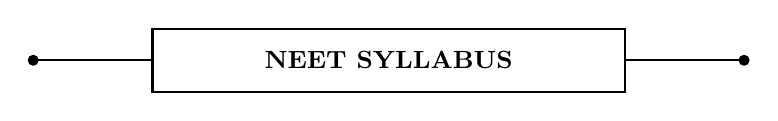
\begin{tikzpicture}
			\node[draw, thick, rectangle, minimum width=6cm, minimum height=0.8cm, align=center, font=\bfseries\small] (title) {NEET SYLLABUS};
			\draw[thick] ([xshift=-1.5cm]title.west) -- (title.west);
			\draw[thick] (title.east) -- ([xshift=1.5cm]title.east);
			\fill ([xshift=-1.5cm]title.west) circle (2pt);
			\fill ([xshift=1.5cm]title.east) circle (2pt);
		\end{tikzpicture}
	\end{center}
	
	\vspace{1em}
	
	% Syllabus Content (italic, justified, small spacing)
	\noindent
	\begin{minipage}[t]{\textwidth}
		\itshape\small
		Electric charges and their conservation. Coulomb’s law–force between two point charges, forces between multiple charges; superposition principle and continuous charge distribution. Electric field, electric field due to a point charge, electric field lines; electric dipole, electric field due to a dipole; torque on a dipole in a uniform electric field. Electric flux, statement of Gauss’s theorem and its applications to find field due to infinitely long straight wire, uniformly charged infinite plane sheet and uniformly charged thin spherical shell (field inside and outside).
		
		\vspace{0.5em}
		
		Electric potential, potential difference, electric potential due to a point charge, a dipole and system of charges: equipotential surfaces, electrical potential energy of a system of two point charges and of electric dipoles in an electrostatic field. Conductors and insulators, free charges and bound charges inside a conductor.
	\end{minipage}
	
\end{frame}

% =============================================================================
% JEE MAIN & ADVANCED SYLLABUS SLIDE
% =============================================================================
\begin{frame}[t]
	\frametitle{}
	\setbeamercovered{transparent=15}
	
	% Header: JEE MAIN & ADVANCED SYLLABUS with diamond bullets
	\noindent
	\begin{center}
		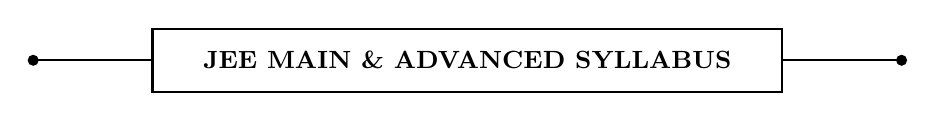
\begin{tikzpicture}
			\node[draw, thick, rectangle, minimum width=8cm, minimum height=0.8cm, align=center, font=\bfseries\small] (title) {JEE MAIN \& ADVANCED SYLLABUS};
			\draw[thick] ([xshift=-1.5cm]title.west) -- (title.west);
			\draw[thick] (title.east) -- ([xshift=1.5cm]title.east);
			\fill ([xshift=-1.5cm]title.west) circle (2pt);
			\fill ([xshift=1.5cm]title.east) circle (2pt);
		\end{tikzpicture}
	\end{center}
	
	\vspace{1em}
	
	% Syllabus Content (italic, justified, small spacing)
	\noindent
	\begin{minipage}[t]{\textwidth}
		\itshape\footnotesize
		\textbf{Electrostatics:} Electric charges and their conservation. Coulomb's law - force between two point charges, forces between multiple charges; superposition principle and continuous charge distribution. Electric field, electric field due to a point charge, electric field lines, electric dipole, electric field due to a dipole, torque on a dipole in uniform electric field.
		
		\vspace{0.4em}
		
		Electric flux, statement of Gauss's theorem and its applications to find field due to infinitely long straight wire, uniformly charged infinite plane sheet and uniformly charged thin spherical shell (field inside and outside). Electric potential, potential difference, electric potential due to a point charge, a dipole and system of charges; equipotential surfaces, electrical potential energy of a system of two point charges and of electric dipole in an electrostatic field.
		
		\vspace{0.4em}
		
		Conductors and insulators, free charges and bound charges inside a conductor. Dielectrics and electric polarization, capacitors and capacitance, combination of capacitors in series and in parallel, capacitance of a parallel plate capacitor with and without dielectric medium between the plates, energy stored in a capacitor.
	\end{minipage}
	
\end{frame}

% =============================================================================
% BOARD SYLLABUS (CBSE/BSEB) SLIDE
% =============================================================================
\begin{frame}[t]
	\frametitle{}
	\setbeamercovered{transparent=15}
	
	% Header: BOARD SYLLABUS with diamond bullets
	\noindent
	\begin{center}
		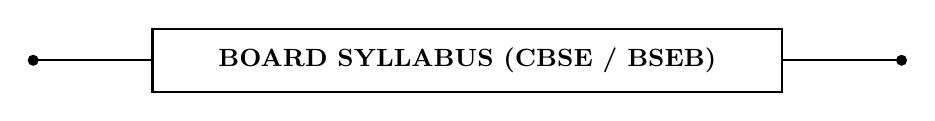
\begin{tikzpicture}
			\node[draw, thick, rectangle, minimum width=8cm, minimum height=0.8cm, align=center, font=\bfseries\small] (title) {BOARD SYLLABUS (CBSE / BSEB)};
			\draw[thick] ([xshift=-1.5cm]title.west) -- (title.west);
			\draw[thick] (title.east) -- ([xshift=1.5cm]title.east);
			\fill ([xshift=-1.5cm]title.west) circle (2pt);
			\fill ([xshift=1.5cm]title.east) circle (2pt);
		\end{tikzpicture}
	\end{center}
	
	\vspace{1em}
	
	% Syllabus Content (italic, justified, small spacing)
	\noindent
	\begin{minipage}[t]{\textwidth}
		\itshape\footnotesize
		\textbf{Chapter 1: Electric Charges and Fields}
		
		\vspace{0.3em}
		
		Electric charges; Conservation of charge, Coulomb's law - force between two point charges, forces between multiple charges; superposition principle and continuous charge distribution. Electric field, electric field due to a point charge, electric field lines; electric dipole, electric field due to a dipole; torque on a dipole in a uniform electric field.
		
		\vspace{0.4em}
		
		Electric flux, statement of Gauss's theorem and its applications to find field due to infinitely long straight wire, uniformly charged infinite plane sheet and uniformly charged thin spherical shell (field inside and outside).
		
		\vspace{0.4em}
		
		\textbf{Chapter 2: Electrostatic Potential and Capacitance}
		
		\vspace{0.3em}
		
		Electric potential, potential difference, electric potential due to a point charge, a dipole and system of charges; equipotential surfaces, electrical potential energy of a system of two point charges and of electric dipole in an electrostatic field. Conductors and insulators, free charges and bound charges inside a conductor. Dielectrics and electric polarization, capacitors and capacitance, combination of capacitors in series and in parallel, capacitance of a parallel plate capacitor with and without dielectric medium between the plates, energy stored in a capacitor, Van de Graaff generator.
	\end{minipage}
	
\end{frame}

\begin{frame}[t]
	\frametitle{}
	\setbeamercovered{transparent=15}
	
	% Title: Name + Lifespan
	\noindent
	\textbf{Charles Augustin de Coulomb (1736 – 1806)}
	
	\vspace{0.5em}
	
	% Body text + Portrait
	\noindent
	\begin{minipage}[t]{0.7\textwidth}
		\small
		Coulomb, a French physicist, began his career as a military engineer in the west Indies. In 1776, he returned to Paris and retired to a small estate to do his scientific research. He invented a torsion balance to measure the quantity of a force and used it for determination of forces of electric attraction or repulsion between small charged spheres. He thus arrived in 1785 at the inverse square law relation, now known as Coulomb's law.
	\end{minipage}%
	\hfill
	\begin{minipage}[t]{0.25\textwidth}
		\centering
		% Fixed: removed image or use placeholder
		\textcolor{gray}{\small [Coulomb Portrait]}
		\vspace{-0.5em}
		\hrule height 0.5pt
		\vspace{0.2em}
		\scriptsize \textit{Charles Augustin de Coulomb}
	\end{minipage}
	
\end{frame}
\begin{frame}[t]
	\frametitle{}
	\setbeamercovered{transparent=15}
	
	% Title: Name + Lifespan
	\noindent
	\textbf{Karl Friedrich Gauss (1777–1855)}
	
	\vspace{0.5em}
	
	% Body text + Portrait
	\noindent
	\begin{minipage}[t]{0.7\textwidth}
		\small
		He was a child prodigy and was gifted in mathematics, physics, engineering, astronomy and even land surveying. The properties of numbers fascinated him, and in his work he anticipated major mathematical development of later times. Along with Wilhelm Welser, he built the first electric telegraph in 1833. His mathematical theory of curved surface laid the foundation for the later work of Riemann.
	\end{minipage}%
	\hfill
	\begin{minipage}[t]{0.25\textwidth}
		\centering
		% Fixed: removed image or use placeholder
		\textcolor{gray}{\small [Gauss Portrait]}
		\vspace{-0.5em}
		\hrule height 0.5pt
		\vspace{0.2em}
		\scriptsize \textit{Karl Friedrich Gauss}
	\end{minipage}
	
\end{frame}
\begin{frame}[t]
	\frametitle{}
	\setbeamercovered{transparent=15}
	
	% Main Title: ELECTROSTATICS
	\noindent
	\begin{center}
		\Large\bfseries ELECTROSTATICS \\
		\vspace{0.3em}
		\hrule height 1.5pt width 0.8\textwidth
	\end{center}
	
	\vspace{1em}
	
	% Section Header: 1. ELECTRIC CHARGE
	\noindent
	\textbf{1. ELECTRIC CHARGE}
	
	\vspace{0.5em}
	
	% Body Text
	\noindent
	\small
	Charge is the property associated with matter due to which it produces and experiences electrical and magnetic effects. The excess or deficiency of electrons in a body is the cause of net charge on a body.
	
	\vspace{0.5em}
	
	\noindent
	\textbf{Types of charge :}
	
	\begin{enumerate}[(i)]
		\item \textbf{Positive charge} : It is the deficiency of electrons as compared to protons.
		\item \textbf{Negative charge} : It is the excess of electrons as compared to protons.
	\end{enumerate}
	
	\vspace{0.5em}
	
	\noindent
	\textbf{SI unit of charge} : ampere × second i.e. coulomb; Dimension : [A T]
	
	\vspace{0.2em}
	
	\noindent
	\textbf{Practical units of charge} are ampere × hour (=3600 C) and faraday (=96500 C)
	
	\vspace{0.7em}
	
	% Bullet Points
	\begin{itemize}
		\item Millikan determined quanta of charge and estimated it to be equal to charge of electron.
		\item 1 C = $3 \times 10^9$ stat coulomb, 1 absolute - coulomb = 10 C, 1 Faraday = 96500 C.
	\end{itemize}
	
	\vspace{0.5em}
	
	% Note Box (bold label)
	\noindent
	\textbf{Note :} Charge of fundamental particles (i.e. electron, proton etc.) is their internal characteristic while charge on a body depends on the number of protons \& electrons inside the body.
	
\end{frame}
\begin{frame}[t]
	\frametitle{}
	\setbeamercovered{transparent=15}
	
	% Section Header
	\noindent
	\textbf{1.1 Specific Properties of Charge}
	
	\vspace{0.7em}
	
	% Main Bullet Points
	\begin{itemize}
		\item \textbf{Charge is a scalar quantity} : It represents excess or deficiency of electrons.
		
		\item \textbf{Charge is transferable} : If a charged body is put in contact with another body, then charge can be transferred to another body.
		
		\item \textbf{Charge is always associated with mass} \\
		Charge cannot exist without mass though mass can exist without charge.
		
		\vspace{0.3em}
		\begin{itemize}
			\item So the presence of charge itself is a convincing proof of existence of mass.
			\item The mass of a body changes after being charged.
			\item When a body is given a positive charge, its mass decreases.
			\item When a body is given a negative charge, its mass increases.
		\end{itemize}
	\end{itemize}
	
\end{frame}
\begin{frame}[t]
	\frametitle{}
	\setbeamercovered{transparent=15}
	
	% Main Content
	\begin{itemize}
		\item \textbf{Charge is quantised} \\
		The quantization of electric charge is the property by virtue of which all free charges are integral multiple of a basic unit of charge represented by $e$. Thus charge $q$ of a body is always given by
		
		\vspace{0.5em}
		\[
		q = ne \qquad \text{where } n = \text{positive or negative integer}
		\]
		
		\vspace{0.5em}
		The quantum of charge is the charge that an electron or proton carries.
		
		\vspace{0.3em}
		\textbf{Note :} Charge on a proton = $(-)$ charge on an electron = $1.6 \times 10^{-19}\,\text{C}$
		
		\vspace{1em}
		
		\item \textbf{Charge is conserved} \\
		In an isolated system, total charge does not change with time though individual charge may change, i.e. charge can neither be created nor destroyed. Conservation of charge is also found to hold good in all types of reactions either chemical (atomic) or nuclear. No exceptions to the rule have ever been found.
	\end{itemize}
	
\end{frame}
\begin{frame}[t]
	\frametitle{}
	\setbeamercovered{transparent=15}
	
	% Main Content with Animation
	\begin{itemize}
		\item<+-> \textbf{Charge is quantised} \\
		The quantization of electric charge is the property by virtue of which all free charges are integral multiple of a basic unit of charge represented by $e$. Thus charge $q$ of a body is always given by
		
		\vspace{0.5em}
		\[
		q = ne \qquad \text{where } n = \text{positive or negative integer}
		\]
		
		\vspace{0.5em}
		\pause
		The quantum of charge is the charge that an electron or proton carries.
		
		\vspace{0.3em}
		\pause
		\textbf{Note :} Charge on a proton = $(-)$ charge on an electron = $1.6 \times 10^{-19}\,\text{C}$
		
		\vspace{1em}
		\pause
		
		\item<+-> \textbf{Charge is conserved} \\
		In an isolated system, total charge does not change with time though individual charge may change, i.e. charge can neither be created nor destroyed. Conservation of charge is also found to hold good in all types of reactions either chemical (atomic) or nuclear. No exceptions to the rule have ever been found.
	\end{itemize}
	
\end{frame}
\begin{frame}[t]
	\frametitle{}
	\setbeamercovered{transparent=15}
	
	% Main Bullet Point (Appears First)
	\begin{itemize}
		\item<+-> \textbf{Charge is invariant} \\
		Charge is independent of frame of reference. i.e. charge on a body does not change whatever be its speed.
		
		\vspace{0.7em}
		
		% Subheading with Animation
		\item<+-> \textbf{Accelerated charge radiates energy}
	\end{itemize}
	\vspace{0.5em}
	
	% Table with Animated Columns
	\noindent
	\begin{tabular}{|c|c|c|}
		\hline
		\onslide<+->{%
			\begin{minipage}[t]{0.28\textwidth}
				\centering
				$v = 0$ (i.e. at rest) \\[0.5em]
				$\oplus$ \\ Q \\[0.5em]
				produces only $\vec{E}$ \\ (electric field)
		\end{minipage}} &
		\onslide<+->{%
			\begin{minipage}[t]{0.28\textwidth}
				\centering
				$v = \text{constant}$ \\[0.5em]
				$\oplus \rightarrow$ \\ Q \\[0.5em]
				produces both $\vec{E}$ and $\vec{B}$ \\ (magnetic field) \\ but no radiation
		\end{minipage}} &
		\onslide<+->{%
			\begin{minipage}[t]{0.28\textwidth}
				\centering
				$v \neq \text{constant}$ (i.e. time varying) \\[0.5em]
				$\oplus \rightarrow$ \\ Q \\[0.5em]
				produces $\vec{E}$, $\vec{B}$ \\ and radiates energy
		\end{minipage}} \\
		\hline
	\end{tabular}
	
\end{frame}
\begin{frame}[t]
	\frametitle{}
	\setbeamercovered{transparent=15}
	
	% Set font to Times New Roman / Serif
	
	% Section Header
	\noindent
	\textbf{1.2 Conductors \& Insulators}
	
	\vspace{0.7em}
	
	% Animated Bullet Points
	\begin{itemize}
		\item<+-> \textbf{Conductors} : Materials in which the outer electrons of each atom or molecule are weakly bound and these electrons are almost free to move throughout the body of the material are known as conductors.
		
		\vspace{0.5em}
		
		\item<+-> \textbf{Insulators} : Materials in which all the electrons are tightly bound to their respective atoms or molecules are known as insulators. In insulators there are very few free electrons. Such materials are also called dielectrics.
		
		\vspace{0.5em}
		
		\item<+-> \textbf{Semiconductors} : Materials whose electrical conductivity lies between that of conductors and insulators. At low temperatures, they behave like insulators; at higher temperatures or under external excitation (e.g., light, heat, doping), they allow some electron flow. Examples: Silicon, Germanium. Their conductivity can be precisely controlled — making them essential for modern electronics.
	\end{itemize}

\end{frame}
\begin{frame}[t]
	\frametitle{}
	\setbeamercovered{transparent=15}
	
	% Set font to Times New Roman / Serif
	
	% Title: Name + Lifespan
	\noindent
	\textbf{Charles Augustin de Coulomb (1736 – 1806)}
	
	\vspace{0.5em}
	
	% Body text + Portrait
	\noindent
	\begin{minipage}[t]{0.7\textwidth}
		\small
		Coulomb, a French physicist, began his career as a military engineer in the west Indies. In 1776, he returned to Paris and retired to a small estate to do his scientific research. He invented a torsion balance to measure the quantity of a force and used it for determination of forces of electric attraction or repulsion between small charged spheres. He thus arrived in 1785 at the inverse square law relation, now known as Coulomb's law.
	\end{minipage}%
	\hfill
	\begin{minipage}[t]{0.25\textwidth}
		\centering
		% Fixed: removed image or use placeholder
		\textcolor{gray}{\small [Coulomb Portrait]}
		\vspace{-0.5em}
		\hrule height 0.5pt
		\vspace{0.2em}
		\scriptsize \textit{Charles Augustin de Coulomb}
	\end{minipage}
	
\end{frame}
\begin{frame}[t]
	\frametitle{}
	\setbeamercovered{transparent=15}
	
	% Title: Name + Lifespan
	\noindent
	\textbf{Karl Friedrich Gauss (1777–1855)}
	
	\vspace{0.5em}
	
	% Body text + Portrait
	\noindent
	\begin{minipage}[t]{0.7\textwidth}
		\small
		He was a child prodigy and was gifted in mathematics, physics, engineering, astronomy and even land surveying. The properties of numbers fascinated him, and in his work he anticipated major mathematical development of later times. Along with Wilhelm Welser, he built the first electric telegraph in 1833. His mathematical theory of curved surface laid the foundation for the later work of Riemann.
	\end{minipage}%
	\hfill
	\begin{minipage}[t]{0.25\textwidth}
		\centering
		% Fixed: removed image or use placeholder
		\textcolor{gray}{\small [Gauss Portrait]}
		\vspace{-0.5em}
		\hrule height 0.5pt
		\vspace{0.2em}
		\scriptsize \textit{Karl Friedrich Gauss}
	\end{minipage}
	
\end{frame}

% ====== OPTIONAL: Add slide transition before this slide ======
\transfade[duration=0.5]

\begin{frame}[t]
\frametitle{}
\setbeamercovered{transparent=15}

% === WATERMARK REMOVED AS REQUESTED ===

% Main Title: "ELECTROSTATICS" (Large, Bold, Centered)
\noindent
\begin{center}
    \Huge\bfseries ELECTROSTATICS
\end{center}

\vspace{1em}

% NEET SYLLABUS Box (Gray background, white text)
\noindent
\colorbox{gray!80}{%
    \parbox[c][1.2cm][c]{0.95\textwidth}{%
        \centering\color{white}\large\bfseries NEET SYLLABUS
    }%
}

\vspace{1em}
\end{frame}
 
\begin{frame}[t]
\begin{itemize}
\item<+-> Electric charges and their conservation.
    \item<+-> Coulomb's law – force between two point charges, forces between multiple charges; superposition principle and continuous charge distribution.
    \item<+-> Electric field, electric field due to a point charge, electric field lines.
    \item<+-> Electric dipole, electric field due to a dipole; torque on a dipole in a uniform electric field.
    \item<+-> Electric flux, statement of Gauss's theorem and its applications to find field due to:
    \begin{itemize}
        \item<+-> Infinitely long straight wire
        \item<+-> Uniformly charged infinite plane sheet
        \item<+-> Uniformly charged thin spherical shell (field inside and outside)
    \end{itemize}
    \item<+-> Electric potential, potential difference, electric potential due to a point charge, a dipole and system of charges.
    \item<+-> Equipotential surfaces, electrical potential energy of a system of two point charges and of electric dipoles in an electrostatic field.
    \item<+-> Conductors and insulators, free charges and bound charges inside a conductor.
\end{itemize}
\end{frame}

% ====== OPTIONAL: Add slide transition before this slide ======
\transfade[duration=0.5]

\begin{frame}[t]
\frametitle{}
\setbeamercovered{transparent=15}

% === WATERMARK REMOVED AS REQUESTED ===

% Title: Name + Lifespan
\noindent
\textbf{Charles Augustin de Coulomb (1736 – 1806)}

\vspace{0.7em}

% Body Text (Animated)
\item<+-> Coulomb, a French physicist, began his career as a military engineer in the west Indies. In 1776, he returned to Paris and retired to a small estate to do his scientific research.

    \vspace{0.5em}
    \pause
    \item<+-> He invented a torsion balance to measure the quantity of a force and used it for determination of forces of electric attraction or repulsion between small charged spheres.

    \vspace{0.5em}
    \pause
    \item<+-> He thus arrived in 1785 at the inverse square law relation, now known as Coulomb’s law. The law had been anticipated by Priestley and also by Cavendish earlier, though Cavendish never published his results.

    \vspace{0.5em}
    \pause
    \item<+-> Coulomb also found the inverse square law of force between unlike and like magnetic poles.

\vspace{1em}

% Optional: Portrait (Replace with actual file if available)
\begin{center}
\onslide<+->{%
\includegraphics[width=0.3\textwidth]{coulomb-portrait.jpg} % Replace with actual file
\vspace{-0.5em}
\hrule height 0.5pt
\vspace{0.2em}
\scriptsize \textit{Charles Augustin de Coulomb}
}
\end{center}

\end{frame}
% ====== OPTIONAL: Add slide transition before this slide ======
\transfade[duration=0.5]

\begin{frame}[t]
\frametitle{}
\setbeamercovered{transparent=15}

% Set font to Times New Roman / Serif
\usefonttheme{serif}
\renewcommand{\familydefault}{\rmdefault}

% === WATERMARK REMOVED AS REQUESTED ===

% Title: Name + Lifespan
\noindent
\textbf{Karl Friedrich Gauss (1777–1855)}

\vspace{0.7em}

% Body Text (Animated)
\item<+-> He was a child prodigy and was gifted in mathematics, physics, engineering, astronomy and even land surveying.

    \vspace{0.5em}
    \pause
    \item<+-> The properties of numbers fascinated him, and in his work he anticipated major mathematical development of later times.

    \vspace{0.5em}
    \pause
    \item<+-> Along with Wilhelm Welser, he built the first electric telegraph in 1833.

    \vspace{0.5em}
    \pause
    \item<+-> His mathematical theory of curved surface laid the foundation for the later work of Riemann.

    \vspace{0.5em}
    \pause
    \item<+-> In physics, his (Gauss’) law is formulated in 1835, but was not published until 1867.

\vspace{1em}

% Optional: Portrait (Replace with actual file if available)
\begin{center}
\onslide<+->{%
\includegraphics[width=0.3\textwidth]{gauss-portrait.jpg} % Replace with actual file
\vspace{-0.5em}
\hrule height 0.5pt
\vspace{0.2em}
\scriptsize \textit{Karl Friedrich Gauss}
}
\end{center}

\end{frame}
% ====== OPTIONAL: Add slide transition before this slide ======
\transfade[duration=0.5]

\begin{frame}[t]
\frametitle{}
\setbeamercovered{transparent=15}

% Set font to Times New Roman / Serif
\usefonttheme{serif}
\renewcommand{\familydefault}{\rmdefault}

% === WATERMARK REMOVED AS REQUESTED ===

% Section Header
\noindent
\textbf{1. ELECTRIC CHARGE}

\vspace{0.7em}

% Definition Paragraph (Appears First)
\noindent
\small
Charge is the property associated with matter due to which it produces and experiences electrical and magnetic effects. The excess or deficiency of electrons in a body is the cause of net charge on a body.

\vspace{0.7em}

% Types of charge (Appears Next)
\noindent
\textbf{Types of charge :}

\begin{enumerate}[(i)]
    \item<+-> \textbf{Positive charge} : It is the deficiency of electrons as compared to protons.
    \item<+-> \textbf{Negative charge} : It is the excess of electrons as compared to protons.
\end{enumerate}

\vspace{0.7em}

% SI unit (Appears Next)
\noindent
\textbf{SI unit of charge} : ampere × second i.e. coulomb; Dimension : [A T]

\vspace{0.2em}
\noindent
\textbf{Practical units of charge} are ampere × hour (=3600 C) and faraday (=96500 C)

\vspace{0.7em}

% Bullet Points (Appears Next)
\item<+-> Millikan determined quanta of charge and estimated it to be equal to charge of electron.
    \item<+-> 1 C = $3 \times 10^9$ stat coulomb, 1 absolute - coulomb = 10 C, 1 Faraday = 96500 C.

\vspace{0.7em}

% Note Box (Appears Last)
\noindent
\textbf{Note :} Charge of fundamental particles (i.e. electron, proton etc.) is their internal characteristic while charge on a body depends on the number of protons \& electrons inside the body.

\end{frame}

% =============================================================================
% ADDITIONAL SLIDES FOR CHAPTER 1 - CONTINUATION
% =============================================================================

\begin{frame}[t]
\frametitle{}
\setbeamercovered{transparent=15}

% Set font to Times New Roman / Serif
\usefonttheme{serif}
\renewcommand{\familydefault}{\rmdefault}

% === WATERMARK REMOVED AS REQUESTED ===

% Section Header
\noindent
\textbf{1.1 Specific Properties of Charge}

\vspace{0.7em}

% Main Bullet Points (Animated)
\item<+-> \textbf{Charge is a scalar quantity} : It represents excess or deficiency of electrons.

    \vspace{0.5em}
    \pause
    \item<+-> \textbf{Charge is transferable} : If a charged body is put in contact with an another body, then charge can be transferred to another body.

    \vspace{0.5em}
    \pause
    \item<+-> \textbf{Charge is always associated with mass} \\
    Charge cannot exist without mass though mass can exist without charge.
    
    \vspace{0.3em}
    \begin{itemize}
        \item<+-> So the presence of charge itself is a convincing proof of existence of mass.
        \item<+-> The mass of a body changes after being charged.
        \item<+-> When a body is given a positive charge, its mass decreases.
        \item<+-> When a body is given a negative charge, its mass increases.
\end{itemize}

\begin{frame}[t]
\frametitle{}
\setbeamercovered{transparent=15}

% Section Header
\noindent
\textbf{1.2 Conductors \& Insulators}

\vspace{0.7em}

% Conductors Definition (Appears First)
\noindent
\textbf{Conductors} : Materials in which the outer electrons of each atom or molecule are weakly bound and these electrons are almost free to move throughout the body of the material are known as conductors.

\vspace{0.7em}

% Insulators Definition (Appears Next)
\noindent
\textbf{Insulators} : Materials in which all the electrons are tightly bound to their respective atoms or molecules are known as insulators. In insulators there are very few free electrons. Such materials are also called dielectrics.

\begin{frame}[t]
\frametitle{}
\setbeamercovered{transparent=15}

% Section Header
\noindent
\textbf{1.3 Methods of Charging}

\vspace{0.7em}

% Friction (Appears First)
\item<+-> \textbf{Friction} \\
    If we rub one body with another body, electrons are transferred from one body to the other.

    \vspace{0.7em}

    % Table (Appears Next)
    \pause
    \noindent
    \begin{tabular}{|l|l|}
        \hline
        \rowcolor{gray!20}
        \textbf{Positive charge} & \textbf{Negative charge} \\
        \hline
        Glass rod & Silk cloth \\
        Woolen cloth & Rubber shoes, Amber, Plastic objects \\
        Dry hair & Comb \\
        Cat skin & Ebonite rod \\
        \hline
        \rowcolor{gray!10}
        \multicolumn{2}{|l|}{\textbf{Note :} Clouds get charged due to friction} \\
        \hline
    \end{tabular}

\begin{frame}[t]
\frametitle{}
\setbeamercovered{transparent=15}

% Section Header
\noindent
\textbf{1.3 Methods of Charging}

\vspace{0.7em}

% Electrostatic Induction (Appears First)
\item<+-> \textbf{Electrostatic induction} \\
    If a charged body is brought near a neutral body, the charged body will attract opposite charge and repel similar charge present in the neutral body. As a result, one side of the neutral body becomes negative while the other positive — this process is called 'electrostatic induction'. Hence induction is a phenomenon of redistribution of charge on a body when any other charged body is brought near it.

    \vspace{0.7em}

    % Charging by Induction Steps (Appears Next)
    \pause
    \noindent
    \textbf{Charging a body by induction (in four successive steps)} \\
    \begin{center}
    \begin{tabular}{cccc}
        \onslide<+->{
        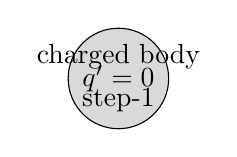
\begin{tikzpicture}[scale=0.5]
            \node[circle,draw,fill=gray!30] (q) at (0,0) {$q'=0$};
            \node[above] at (q) {charged body};
            \node[below] at (q) {step-1};
        \end{tikzpicture}} &
        \onslide<+->{
        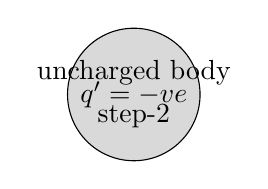
\begin{tikzpicture}[scale=0.5]
            \node[circle,draw,fill=gray!30] (q) at (0,0) {$q'=-ve$};
            \node[above] at (q) {uncharged body};
            \node[below] at (q) {step-2};
        \end{tikzpicture}} &
        \onslide<+->{
        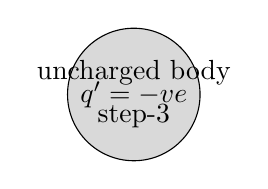
\begin{tikzpicture}[scale=0.5]
            \node[circle,draw,fill=gray!30] (q) at (0,0) {$q'=-ve$};
            \node[above] at (q) {uncharged body};
            \node[below] at (q) {step-3};
        \end{tikzpicture}} &
        \onslide<+->{
        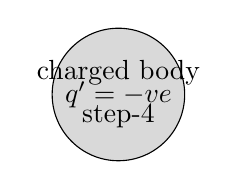
\begin{tikzpicture}[scale=0.5]
            \node[circle,draw,fill=gray!30] (q) at (0,0) {$q'=-ve$};
            \node[above] at (q) {charged body};
            \node[below] at (q) {step-4};
        \end{tikzpicture}} \\
    \end{tabular}
    \end{center}

    \vspace{0.7em}

    % Notes on Induction (Appears Last)
    \pause
    \noindent
    \textbf{In case of induction it is worth noting that:}
    \begin{enumerate}[(i)]
        \item<+-> Inducing body neither gains nor loses charge.
        \item<+-> The nature of induced charge is always opposite to that of inducing charge.
        \item<+-> Induced charge can be lesser or equal to inducing charge (but never greater).
        \item<+-> Induction takes place only in bodies (either conducting or non conducting) and not in particles.
    \end{enumerate}

\end{frame}
% ====== OPTIONAL: Add slide transition before this slide ======
\transfade[duration=0.5]

\begin{frame}[t]
\frametitle{}
\setbeamercovered{transparent=15}

% Set font to Times New Roman / Serif
\usefonttheme{serif}
\renewcommand{\familydefault}{\rmdefault}

% === WATERMARK REMOVED AS REQUESTED ===

% Section Header
\noindent
\textbf{1.3 Methods of Charging}

\vspace{0.7em}

% Conduction (Appears First)
\item<+-> \textbf{Conduction} \\
    The process of transfer of charge by contact of two conducting bodies is known as conduction.

    \vspace{0.5em}
    \pause
    If a charged conducting body is put in contact with uncharged conducting body, the uncharged body becomes charged due to transfer of electrons from one body to the other.

    \vspace{0.5em}
    \pause
    The charged body loses some of its charge (which is equal to the charge gained by the uncharged body).

\begin{frame}[t]
\frametitle{}
\setbeamercovered{transparent=15}

% Header: GOLDEN KEY POINTS (Black Bar, White Text)
\noindent
\begin{center}
    \colorbox{black}{\parbox[c][0.8cm][c]{0.8\textwidth}{\centering\color{white}\large\bfseries GOLDEN KEY POINTS}}
\end{center}

\vspace{1em}

% Content List (Animated)
\item<+-> \textbf{Charge differs from mass in the following aspects :}
    \begin{enumerate}[(i)]
        \item<+-> In SI units, charge is a derived physical quantity while mass is a fundamental quantity.
        \item<+-> Charge is always conserved but mass is not.
        \item<+-> Charge cannot exist without mass but mass can exist without charge.
        \item<+-> Charges are of two type (positive and negative) but mass is of only one type (positive).
        \item<+-> For a moving charged body, mass increases while charge remains constant.
    \end{enumerate}

    \vspace{0.7em}

    \item<+-> \textbf{True test of electrification is repulsion} and not attraction as attraction can take place between a charged and an uncharged body or between two similarly charged bodies.

    \vspace{0.7em}

    \item<+-> \textbf{For a non relativistic (i.e. $v << c$) charged particle}, specific charge $\dfrac{q}{m} = \text{constant}$.

    \vspace{0.7em}

    \item<+-> \textbf{Charge can be detected and/or measured} with the help of gold-leaf electroscope, electrometer, voltmeter etc.
\begin{frame}[t]
\frametitle{}
\setbeamercovered{transparent=15}

% Section Header
\noindent
\textbf{3.1 Intensity of electric field due to point charge}

\vspace{0.7em}

% Definition Paragraph (Appears First)
\noindent
Electric field intensity is defined as force on unit test charge.
\[
\vec{E} = \lim_{q_0 \to 0} \frac{\vec{F}}{q_0} = \frac{kq}{r^2} \hat{r} = \frac{kq}{r^3} \vec{r}
\]

\vspace{0.5em}

% Note on Test Charge (Appears Next)
\onslide<+->{
\textbf{Note:} Test charge ($q_0$) is a fictitious charge that exerts no force on nearby charges but experiences forces due to them.
}

\vspace{0.7em}

% Diagram (Appears Last)
\begin{center}
\onslide<+->{
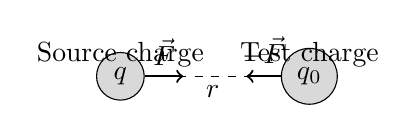
\begin{tikzpicture}[scale=0.8]
    \node[circle,draw,fill=gray!30] (q) at (0,0) {$q$};
    \node[above] at (q) {Source charge};
    \node[circle,draw,fill=gray!30] (q0) at (3,0) {$q_0$};
    \node[above] at (q0) {Test charge};
    \draw[->,thick] (q) -- ++(1,0) node[midway,above] {$\vec{F}$};
    \draw[dashed] (q) -- (q0) node[midway,below] {$r$};
    \draw[->,thick] (q0) -- ++(-1,0) node[midway,above] {$-\vec{F}$};
\end{tikzpicture}}
\end{center}

\end{frame}
\begin{frame}[t]
\frametitle{}
\setbeamercovered{transparent=15}

% Section Header
\noindent
\textbf{3.2 Properties of electric field intensity}

\vspace{0.7em}

% Property (i) (Appears First)
\onslide<+->{
\item \textbf{(i)} It is a vector quantity. Its direction is the same as the force experienced by positive charge.}

\vspace{0.5em}

% Property (ii) (Appears Next)
\onslide<+->{
\item \textbf{(ii)} Electric field due to positive charge is always away from it while due to negative charge it is always towards it.}

\vspace{0.5em}

% Property (iii) (Appears Next)
\onslide<+->{
\item \textbf{(iii)} Its unit is newton/coulomb.}

\vspace{0.5em}

% Property (iv) (Appears Next)
\onslide<+->{
\item \textbf{(iv)} Its dimensional formula is $[MLT^{-3}A^{-1}]$}

\vspace{0.5em}

% Property (v) (Appears Next)
\onslide<+->{
\item \textbf{(v)} Force on a point charge is in the same direction as that of electric field; on positive charge and in opposite direction on a negative charge. \\
    $\vec{F} = q \vec{E}$}

\vspace{0.5em}

% Property (vi) (Appears Last)
\onslide<+->{
\item \textbf{(vi)} It obeys the superposition principle i.e., the field intensity due to a charge distribution is the vector sum of the field intensities due to individual charges at any given point.}

\end{frame}

